\documentclass[a4paper,11pt]{article}
\usepackage[T1]{fontenc}
\usepackage[utf8]{inputenc}
\usepackage{lmodern}
\usepackage{amsmath}
\usepackage{amsfonts}

\usepackage{graphicx}

\title{Assignment \#1 -- Introduction to Robotics}
\author{
Luisa Zintgraf \texttt{6027303} \\
Weipeng He \texttt{6411529} \\
Philipp Ruppel \texttt{6248024}
}

\begin{document}

\maketitle

\section{}
See MATLAB-files ``assignment1task1.m'' and ``plot\_pyramid.m''.
For the solution, simply type
\begin{center}
  \texttt{[V1, V2] = assignment1task1}
\end{center}
into the MATLAB command window and as an output you will get different plots for
visualization as well as matrices V1 and V2, which hold (columnwise) A, B, C, D, E,
M. V1 then holds the coordinates of the solution after rotating the pyramid in the
coordinate frame $M_{uvw}$, and V1 in $M_{xyz}$.

\section{}
The transformation from A to C is the composition of the transformation from A to B and the transformation from B to C, namely : $^AT_C = ^AT_B ~ ^BT_C$

The homogeneous transformations $^AT_B$ and $^BT_C$ both consist of only translation and rotation (no projection). Thus, $^AT_C$ also consists of translation and rotation, so that it is inversible. 

Therefore, the interpretation of the transformation $^AT_C$ can be assumed to be unambiguous.

\section{}
See MATLAB-files ``rotation.m''.

\section{}
We denote the homogeneous transformation using matrix:
\[ \begin{pmatrix}
  \mathbf{R} & \mathbf{t} \\
  \mathbf{0} & 1 
\end{pmatrix} \]
where $\mathbf{R}$ is a 3 by 3 rotation matrix and $\mathbf{t}$ is a 3 by 1 translation vector.
The rotation matrix is a unit orthogonal matrix, that is $\mathbf{R}\mathbf{R}^T=\mathbf{I}$. Thus, we have:

\[
\begin{pmatrix}
  \mathbf{R} & \mathbf{t} \\
  \mathbf{0} & 1 
\end{pmatrix} 
\begin{pmatrix}
  \mathbf{R}^T & -\mathbf{R}^T\mathbf{t} \\
  \mathbf{0} & 1 
\end{pmatrix}
= 
\begin{pmatrix}
  \mathbf{R}\mathbf{R}^T & -\mathbf{R}\mathbf{R}^T\mathbf{t} + \mathbf{t} \\
  \mathbf{0} & 1 
\end{pmatrix}
= 
\begin{pmatrix}
  \mathbf{I} & \mathbf{0} \\
  \mathbf{0} & 1 
\end{pmatrix}
= \mathbf{I}
\]

Therefore $\begin{pmatrix}
  \mathbf{R}^T & -\mathbf{R}^T\mathbf{t} \\
  \mathbf{0} & 1 
\end{pmatrix}$ is the inverse transformation.

\section{}
For solving this task, I assumed that F and M are in the same position at the beginning. Also, I assumed that the point we are talking about is in M, because if it was in F, it wouldn’t move at all. The coordinates in F are $[-1,-3, 0]$ (and in M still $[1, 0, 0]$). 
(If it was meant the other way around, that is that the point is in F and M is moving, the coordinates in F would stay the same and in M, they would be $[-1, 3, 0]$ after the movements).

In this visualization, the blue coordinate frame is F and the red one is M after the translation and the rotation.
\begin{center}
  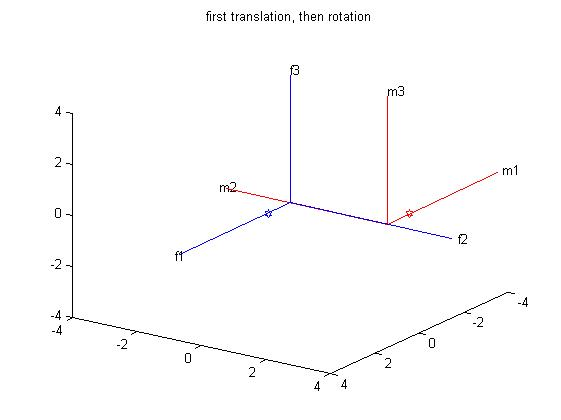
\includegraphics[width=0.8\textwidth]{aufg5}
\end{center}

If the sequence of the operations is reversed, the result should be the same. Since we only rotate and translate in reference to F, the steps can be done in any order. If we had any action in reference to M (e.g. ``translate M along m2 by 3 units''), the results would differ when reversing the sequence of operations.
\end{document}
